% ------------------------------------------------------------------------------
% TYPO3 CMS 8.5 - What's New - Chapter "Introduction" (Dutch Version)
%
% @author	Michael Schams <schams.net>
% @license	Creative Commons BY-NC-SA 3.0
% @link		http://typo3.org/download/release-notes/whats-new/
% @language	English
% ------------------------------------------------------------------------------
% LTXE-CHAPTER-UID:		7fdf26cc-362160ab-d6c8b905-19722b20
% LTXE-CHAPTER-NAME:	Introduction
% ------------------------------------------------------------------------------

\section{Inleiding}
\begin{frame}[fragile]
	\frametitle{Inleiding}

	\begin{center}\huge{Inleiding}\end{center}
	\begin{center}\huge{\color{typo3darkgrey}\textbf{De feiten}}\end{center}

\end{frame}

% ------------------------------------------------------------------------------
% LTXE-SLIDE-START
% LTXE-SLIDE-UID:		b3a54cf3-2f0906e8-acf32ed2-cea4e1e9
% LTXE-SLIDE-ORIGIN:	344cc625-72176049-0721f1aa-0580f11a English
% LTXE-SLIDE-TITLE:		TYPO3 CMS 8.5 - The Facts
% ------------------------------------------------------------------------------
\begin{frame}[fragile]
	\frametitle{Inleiding}
	\framesubtitle{TYPO3 CMS 8.5 - De feiten}

	\begin{itemize}
		\item Publicatiedatum: 20 december 2016
		\item Publicatietype: Sprintrelease
		\item Motto: Op de klok
	\end{itemize}

	\begin{figure}
		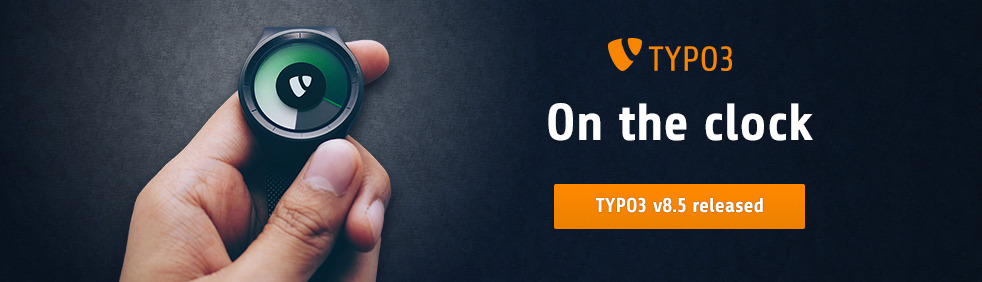
\includegraphics[width=0.95\linewidth]{Introduction/typo3cms85-banner.jpg}
	\end{figure}

\end{frame}

% ------------------------------------------------------------------------------
% LTXE-SLIDE-START
% LTXE-SLIDE-UID:		e9a56d81-56aa16ce-71d72876-31d004d1
% LTXE-SLIDE-ORIGIN:	59b04868-09a761b3-0c7ca4c3-ce6e31bb English
% LTXE-SLIDE-TITLE:		System Requirements
% ------------------------------------------------------------------------------
\begin{frame}[fragile]
	\frametitle{Inleiding}
	\framesubtitle{Systeemeisen}

	\begin{itemize}
		\item PHP:\tabto{2.2cm}versie 7
		\item MySQL:\tabto{2.2cm}versie 5.5 tot 5.7
		\item Schijfruimte:\tabto{2.2cm}min 200 MB
		\item PHP-instellingen:

			\begin{itemize}
				\item \texttt{memory\_limit} >= 128M
				\item \texttt{max\_execution\_time} >= 240s
				\item \texttt{max\_input\_vars} >= 1500
				\item compilatieoptie \texttt{-}\texttt{-disable-ipv6} \underline{niet} gebruiken
			\end{itemize}

		\item De backend vereist Microsoft Internet Explorer 11 of hoger,
			Microsoft Edge, Google Chrome, Firefox, Safari
			of een andere moderne, compatibele browser

	\end{itemize}

\end{frame}

% ------------------------------------------------------------------------------
% LTXE-SLIDE-START
% LTXE-SLIDE-UID:		f3952d29-bd9084a2-97c40c86-0d632282
% LTXE-SLIDE-ORIGIN:	41f1b51a-6b837f9d-c4aa9584-66f8e47f English
% LTXE-SLIDE-TITLE:		Development And Release Timeline
% ------------------------------------------------------------------------------
\begin{frame}[fragile]
	\frametitle{Inleiding}
	\framesubtitle{Ontwikkelings- en publicatietijdlijn}

	\begin{figure}
		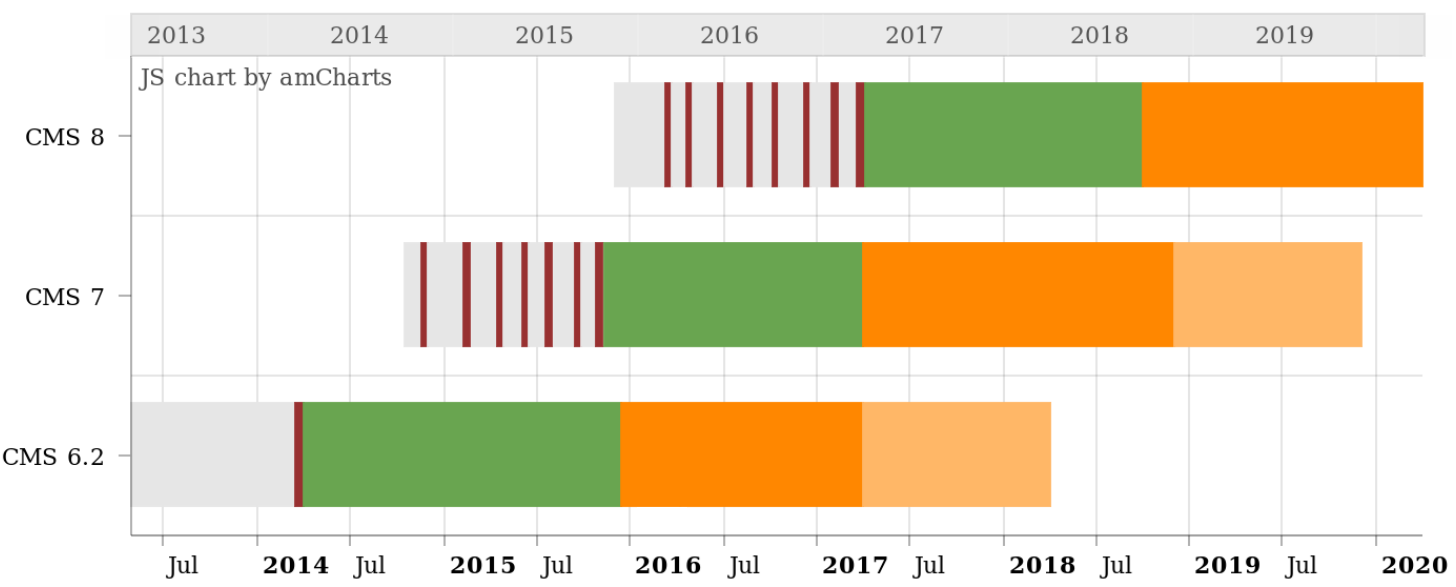
\includegraphics[width=1\linewidth]{Introduction/ReleaseAgenda.png}
	\end{figure}

\end{frame}

% ------------------------------------------------------------------------------
% LTXE-SLIDE-START
% LTXE-SLIDE-UID:		4beb7ea4-e4a81b03-1a3ad306-4064cb19
% LTXE-SLIDE-ORIGIN:	f7c981ac-f359aac8-f8799a73-2adc6532 English
% LTXE-SLIDE-TITLE:		TYPO3 CMS Roadmap
% ------------------------------------------------------------------------------
\begin{frame}[fragile]
	\frametitle{Inleiding}
	\framesubtitle{TYPO3 CMS Roadmap}

	Publicatiedatums en de primaire focus

	\begin{itemize}

		\item v8.0 \tabto{1.1cm}22 mar 2016\tabto{3.4cm}Lastminute toevoegingen
		\item v8.1 \tabto{1.1cm}03 mei 2016\tabto{3.4cm}Cloud-integratie
		\item v8.2 \tabto{1.1cm}05 jul 2016\tabto{3.4cm}Randvoorwaarden Doctrine
		\item v8.3 \tabto{1.1cm}30 aug 2016\tabto{3.4cm}Rich Text Editor
		\item v8.4 \tabto{1.1cm}18 okt 2016\tabto{3.4cm}Doctrine-migratie + upgrades
		\item
			\begingroup
				\color{typo3orange}
					v8.5 \tabto{1.1cm}20 dec 2016\tabto{3.4cm}Nieuwe RTE + Integrator-ondersteuning
			\endgroup
		\item v8.6 \tabto{1.1cm}14 feb 2017\tabto{3.4cm}\textit{nader te bepalen}
		\item v8.7 \tabto{1.1cm}04 apr 2017\tabto{3.4cm}Voorbereiding LTS

	\end{itemize}

	\smaller
		\url{https://typo3.org/typo3-cms/roadmap/}\newline
		\url{https://typo3.org/news/article/kicking-off-typo3-v8-development/}
	\normalsize

\end{frame}

% ------------------------------------------------------------------------------
% LTXE-SLIDE-START
% LTXE-SLIDE-UID:		f831636f-877ce5ab-ac04436c-6df0b9c5
% LTXE-SLIDE-ORIGIN:	425f3f15-1178ed7e-f26438f9-a79ad9e9 English
% LTXE-SLIDE-TITLE:		Installation
% ------------------------------------------------------------------------------
\begin{frame}[fragile]
	\frametitle{Inleiding}
	\framesubtitle{Installatie}

	\begin{itemize}
		\item Officiële \textit{klassieke} installatieprocedure op Linux/Mac OS X\newline
			(DocumentRoot bijvoorbeeld \texttt{/var/www/site/htdocs}):
		\begin{lstlisting}
			$ cd /var/www/site
			$ wget --content-disposition get.typo3.org/8.5
			$ tar xzf typo3_src-8.5.1.tar.gz
			$ cd htdocs
			$ ln -s ../typo3_src-8.5.1 typo3_src
			$ ln -s typo3_src/index.php
			$ ln -s typo3_src/typo3
			$ touch FIRST_INSTALL
		\end{lstlisting}

		\item Symbolische koppelingen op Microsoft Windows:

			\begin{itemize}
				\item Gebruik \texttt{junction} op Windows XP/2000
				\item Gebruik \texttt{mklink} op Windows Vista en Windows 7
			\end{itemize}

	\end{itemize}
\end{frame}

% ------------------------------------------------------------------------------
% LTXE-SLIDE-START
% LTXE-SLIDE-UID:		abfc1d95-0344b90d-782d1d9a-03991aef
% LTXE-SLIDE-ORIGIN:	061ecffe-6aadad2d-6e64a67a-3c50a5cf English
% LTXE-SLIDE-TITLE:		Upgrade to TYPO3 CMS 7
% ------------------------------------------------------------------------------
\begin{frame}[fragile]
	\frametitle{Inleiding}
	\framesubtitle{Upgrade naar TYPO3 CMS 8.x}

	\begin{itemize}
		\item Upgrades alleen mogelijk vanaf TYPO3 CMS 7.6 LTS
		\item TYPO3 CMS < 7.6 LTS moet eerst naar TYPO3 CMS 7.6 LTS bijgewerkt worden
	\end{itemize}

	\begin{itemize}

		\item Instructies voor het upgraden:\newline
			\smaller\url{http://wiki.typo3.org/Upgrade#Upgrading_to_8.5}\normalsize
		\item Officiële TYPO3-handleiding "TYPO3 Installation and Upgrading":
			\smaller\url{http://docs.typo3.org/typo3cms/InstallationGuide}\normalsize
		\item Algemene aanpak:
			\begin{itemize}
				\item Controleer minimale systeemeisen \small(PHP, MySQL, etc.)
				\item Controleer \textbf{deprecation\_*.log} in de oude TYPO3-installatie
				\item Werk alle extensies bij naar de nieuwste versie
				\item Plaats nieuwe broncode en start Installatie-module \textrightarrow Upgrade Wizard
				\item Controleer de startmodule voor backend gebruikers (optioneel)
			\end{itemize}
	\end{itemize}

\end{frame}


% ------------------------------------------------------------------------------
% LTXE-SLIDE-START
% LTXE-SLIDE-UID:		e5c2f72b-72e40465-42919f4c-34d3e1af
% LTXE-SLIDE-ORIGIN:	560abc87-898d82d3-b9e35f84-e348c121 English
% LTXE-SLIDE-TITLE:		PHP Version 7
% ------------------------------------------------------------------------------
\begin{frame}[fragile]
	\frametitle{Inleiding}
	\framesubtitle{PHP Versie 7}

	\begin{itemize}

		\item TYPO3 CMS 8.x vereist minimaal PHP 7.0
		\item TYPO3 zal volgende PHP 7-versies ondersteunen
		\item Deze versie geeft significant betere prestaties op het hele systeem

		\item Niet alleen backendgebruikers ervaren een soepelere interface: het
			nieuwe record voor het laden van een volledig gecachete pagina in de frontend is nu minder
			dan 7 milliseconden, wat ongeveer 40\% sneller is dan met PHP versie 5.5

		\item We zijn reeds begonnen met het gebruiken van nieuwe kenmerken van deze PHP-versie,
			de cryptografisch veilige pseudotoevalsgeneratoren worden bijvoorbeeld al ingezet

	\end{itemize}

\end{frame}

% ------------------------------------------------------------------------------
